\section{System Realization in \system}\label{sec:system}

\subsection{Relevant Runtime Surfaces}

The full repository contains many subsystems, but only a subset is required to support the thesis of this paper. The method described in Section~III is realized through four concrete surfaces.

First, the \textbf{agent gateway} accepts authenticated WebSocket traffic from agents and dashboard clients, applies socket- and user-level rate limits, verifies tenant context, and records audit events. This is the entry point through which distributed evidence reaches the control plane. Second, \textbf{command signing} ensures that response actions sent back to an agent are integrity-protected. Third, the \textbf{platform configuration surface} exposes routing and privacy controls used by the triage layer. Fourth, the \textbf{case-file path} persists the outcome of triage for later inspection.

The resulting system scope is narrower than the overall product scope. Hardware deployment tooling, dashboard visual polish, and general admin functionality are part of the repository, but they are peripheral to the present claim and are therefore not treated as primary research contributions.

\subsection{Distributed Path From Request to Action}

The control path of interest proceeds as follows:
\begin{enumerate}
  \item a distributed agent or gateway-observed request is normalized into a traffic object;
  \item the three-role triage pipeline produces initial role outputs;
  \item disagreement metrics decide whether bounded debate is required;
  \item the final output is synthesized into a verdict distribution and a case file;
  \item if action is required, the control plane dispatches a signed command back to the relevant agent.
\end{enumerate}

This path is intentionally auditable at each transition. The gateway contributes authentication and rate limiting, the command path contributes integrity, and the audit layer contributes retention and verification.

\subsection{Routing and Privacy Modes}

The repository currently exposes route modes including \texttt{cloud\_only}, \texttt{local\_preferred}, and \texttt{hybrid\_verify}. These modes are not presented here as an independent contribution; they serve as deployment support for debate-driven triage. In particular, they allow the system to distinguish between operational latency mode and privacy-sensitive mode. The current validated workspace snapshot reports \texttt{cloud\_only} as the active routing mode and \texttt{privacyMode=off}; this is important because the latency values reported in Section~V are therefore orchestration measurements under the present configuration rather than full local-model inference measurements.

\begin{figure}[t]
  \centering
  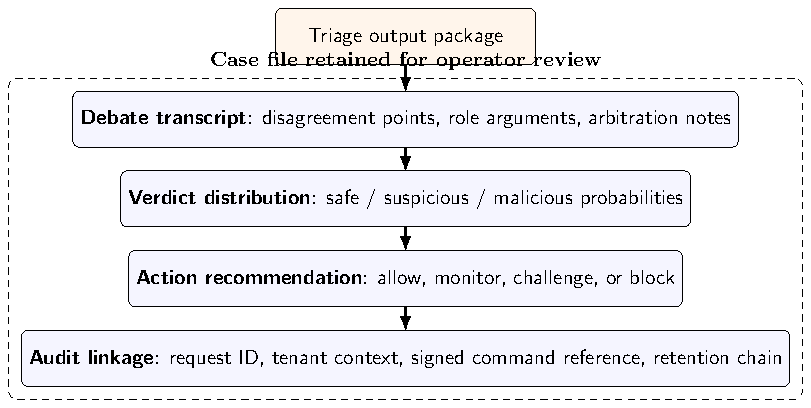
\includegraphics[width=\linewidth]{fig-case-file.pdf}
  \caption{Auditable outputs emphasized in this paper.}
  \label{fig:case-file}
\end{figure}

\subsection{Why the System Claim Stays Conservative}

The repository also includes benchmark harnesses, deployment bundles, device workflows, and whitepaper-style claims. This draft deliberately avoids turning those into broad system-performance promises. The validated workspace snapshot is mixed: it confirms the presence of benchmark infrastructure, audit-chain verification, notification outbox behavior, and device-gateway compatibility, but it does not validate the strongest historical throughput or deployment-scale statements. Therefore, the manuscript uses those artifacts only to support a limited statement: the triage method has been implemented inside a real distributed security platform with authenticated control and measurable overhead, not that every historical platform-scale claim has been reproduced in the current environment.

\subsection{Implementation Boundary for This Draft}

The system realization claim can therefore be stated precisely. \system\ provides:
\begin{itemize}
  \item a concrete three-role triage implementation with disagreement-triggered debate;
  \item authenticated and rate-limited WebSocket control paths;
  \item HMAC-backed command dispatch and auditable event logging;
  \item deployable route modes for local/cloud/hybrid inference decisions.
\end{itemize}
This boundary is sufficient for a JCST-style system-and-method paper focused on multi-agent security judgment, and it avoids the broader platform sprawl that would otherwise dilute the paper.
